\documentclass[11pt]{article}
\usepackage[a4paper,margin=25mm]{geometry}
\usepackage{amsmath,amssymb,graphicx,microtype}
\usepackage[unicode,colorlinks=true,urlcolor=blue,linkcolor=blue]{hyperref}
\setlength{\emergencystretch}{3em}
\title{An evaluated arithmetic pairing for the original endpoint test}
\author{Split-Zero research programme}
\date{23 September 2026}
\begin{document}
\maketitle
\begin{figure}[ht]
\centering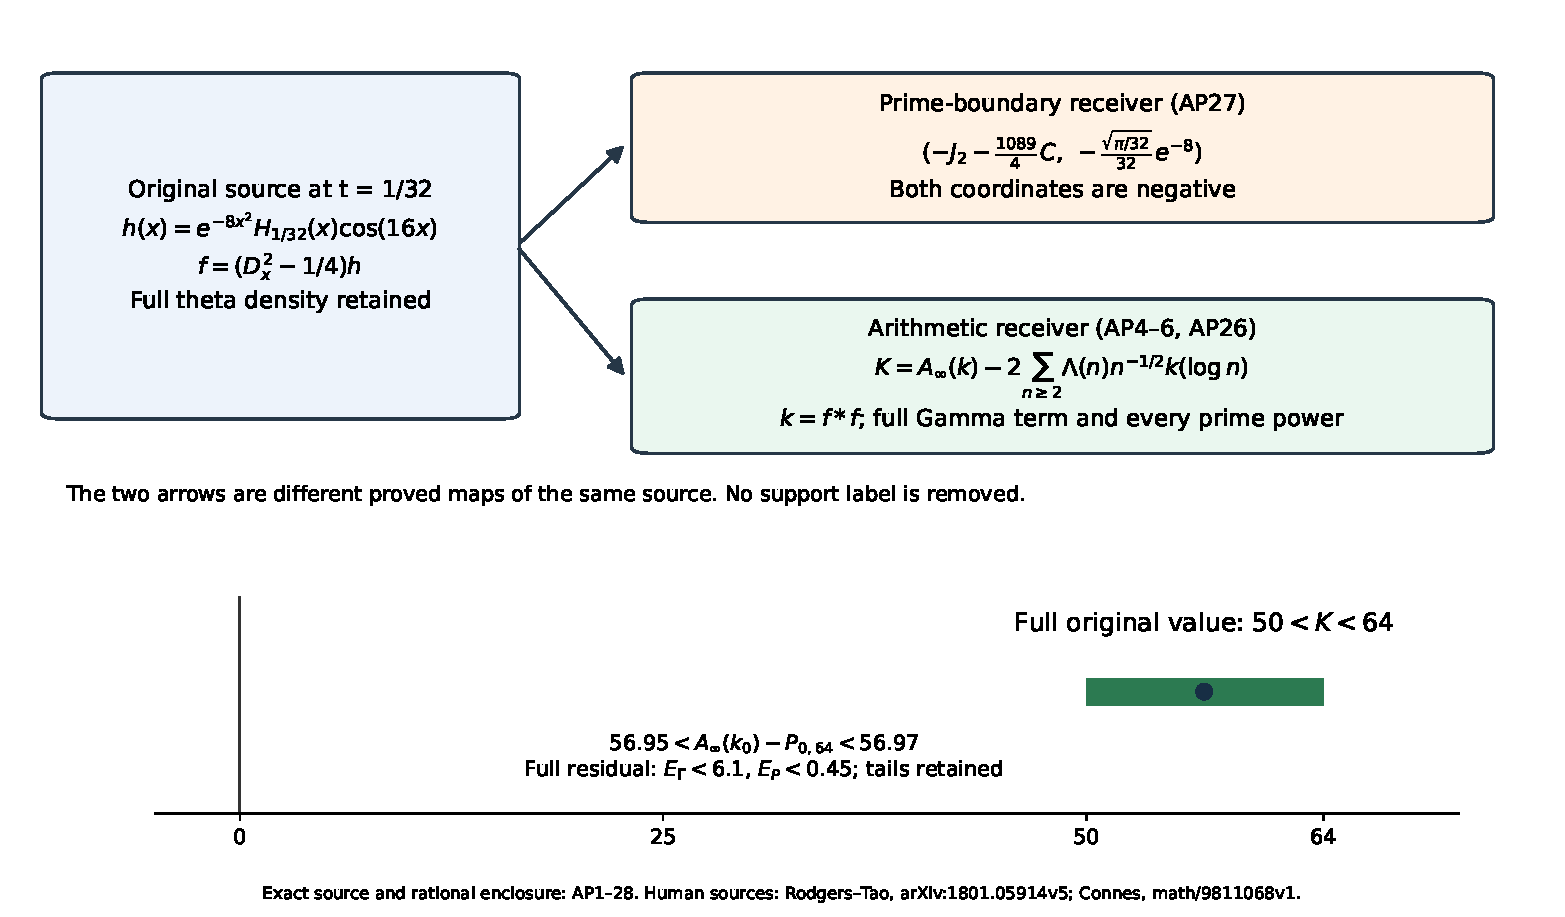
\includegraphics[width=\linewidth]{PAIRING_MAP.pdf}
\caption{The same original source has the two distinct, fully computed
receivers AP27 and AP4--6. The green interval is the certified enclosure
AP1, including the entire residual AP26. The dark point marks the narrow
comparison interval AP25. The diagram displays exact formulas and proved
rational bounds, rather than sampled zeta zeros.}
\end{figure}
\section{The actual endpoint test has a strictly positive arithmetic pairing}

This calculation evaluates the test constructed by the endpoint-resonance
calculation. It uses the original meromorphic Riemann zeta function,
its prime powers, its pole, every trivial zero at each finite contour
cutoff, and the full Gamma boundary. At the original time \(t=1/32\),
the result is the certified rational enclosure
\[
 \boxed{50<K_{1/32}<64.}\tag{AP1}
\]
Here \(K_t\) is defined below for this one explicit test. The two
negative source moments of the same test therefore do not give a
negative Weil pairing. The calculation determines this test's sign;
it does not assert positivity for every test.

\subsection{Original source, coordinates, and zeta factors}
Throughout, \(x,u\) are the original real coordinates and
\(t=1/32\). Retain
\[
\begin{split}
 \Phi(u)&=\sum_{n=1}^\infty
 (2\pi^2n^4e^{9u}-3\pi n^2e^{5u})e^{-\pi n^2e^{4u}},\\
 H(x)&=\int_0^\infty e^{u^2/32}\Phi(u)\cos(xu)\,du,\\
 h(x)&=e^{-8x^2}H(x)\cos(16x),\qquad
 f(x)=h''(x)-\tfrac14h(x),\qquad k=f*f,\\
 F(s)&=\int_{\mathbb R}f(x)e^{-(s-1/2)x}\,dx.
\end{split}\tag{AP2}
\]
The density and heat convention are those of Brad Rodgers and Terence
Tao, \emph{The de Bruijn--Newman constant is non-negative},
\href{https://arxiv.org/abs/1801.05914v5}{version 5}, original TeX
equations \texttt{phidef}, \texttt{htdef}, \texttt{hoz}, and
\texttt{sas}. Only those source formulas are used here; the present
sign calculation uses no assumption about the location of zeta zeros.

For clarity, the test's exact return to the original function is
displayed with every factor. Set \(w=s-1/2\),
\(\sigma_0=itw\), \(\sigma_1=1+itw\). Then
\[
\begin{split}
 F(s)=\frac{s(s-1)\sqrt{\pi t}}{16}\bigl\{&
 e^{t(w-i/(2t))^2}\sigma_1(\sigma_1-1)\pi^{-\sigma_1/2}
       \Gamma(\sigma_1/2)\zeta(\sigma_1)\\
 {}+{}&e^{t(w+i/(2t))^2}\sigma_0(\sigma_0-1)\pi^{-\sigma_0/2}
       \Gamma(\sigma_0/2)\zeta(\sigma_0)\bigr\}.
\end{split}\tag{AP3}
\]
Every product at an exceptional argument is the analytic continuation
of the displayed full product. In particular the products at arguments
zero and one both equal one. The pole of \(\zeta\) at one and
the pole of \(\Gamma(s/2)\) at zero are included in this statement.
To prove AP3, Gaussian integration gives
\[
 \int_{\mathbb R}e^{-x^2/(4t)}H_t(x)e^{-wx}\,dx
 =2\sqrt{\pi t}\,e^{tw^2}H_0(2tw).
\]
The two exponential terms of \(\cos(x/(2t))\), followed by
\(16H_0(z)=s(s-1)\pi^{-s/2}\Gamma(s/2)\zeta(s)\) with
\(s=1/2+iz/2\), give AP3. Absolute interchange follows from the
outer Gaussian and the super-exponential original density. Two
integrations by parts give the retained factor \(s(s-1)\).
Consequently \(F(0)=F(1)=0\), exactly.

\subsection{Complete arithmetic receiver}
Write \(j=\zeta'/\zeta\), and let \(\rho\) run through the
nontrivial zeros of the original function with multiplicity \(m_\rho\).
The exact quantity evaluated is
\[
 K=\sum_\rho m_\rho F(\rho)^2
   =A_\infty(k)-P(k),\qquad
 P(k)=2\sum_{n\ge2}\frac{\Lambda(n)}{\sqrt n}k(\log n),
 \tag{AP4}
\]
where \(\Lambda(p^a)=\log p\) for every prime power and
\(\Lambda(n)=0\) otherwise. The full archimedean term is
\[
 A_\infty(k)=-(\gamma_{\rm E}+\log\pi)k(0)+
 \int_0^\infty\frac{e^{-x}k(0)-e^{-x/4}k(x/2)}{1-e^{-x}}\,dx.
 \tag{AP5}
\]
Evenness and reality give
\(\overline{F(1-\overline s)}=F(s)\). Thus AP4 has the actual
reflected Weil product; away from the critical line it has not been
replaced by an absolute square.

We recall the finite-cutoff derivation to retain the original divisor.
Put \(A=F^2\), \(b_N=-2N-1\),
\(U_N=\sum_{m=1}^N A(-2m)\), and
\(\kappa(s)=-\tfrac12\log\pi+\tfrac12\psi_\Gamma(s/2)\).
For upward vertical integrals \(I_c=(2\pi i)^{-1}\int_{\Re s=c}\),
the argument principle and the full original functional equation give
\[
\begin{split}
 V_N&=K+U_N-A(1)=I_\sigma(Aj)-I_{b_N}(Aj),\quad \sigma>1,\\
 j(s)+j(1-s)&=-\kappa(s)-\kappa(1-s),\\
 V_N&=-P(k)+\mathcal G_N,\\
 \mathcal G_N&=I_{b_N}\{A(s)[\kappa(s)+\kappa(1-s)]\}
             =A_\infty(k)+A(0)+U_N.
\end{split}\tag{AP6}
\]
The rational derivatives of \(s(s-1)\) in the original multiplier
cancel with their reflected partners in the displayed reflection
identity; the pole at one remains explicitly in \(V_N\).
On the right edge \(j(s)=-\sum\Lambda(n)n^{-s}\); Mellin inversion
gives the two prime legs. Moving the Gamma edge to \(1/2\) crosses
exactly the residues at \(0,-2,\ldots,-2N\), giving
\(A(0)+U_N\). The digamma integral on \(1/2\) gives AP5 with
its combined numerator. This proves AP4 because both endpoints vanish.
No limit or finite value is assigned to \(U_N\) individually.

For the classical contour and measure conventions, see Alain Connes,
\emph{Trace formula in noncommutative geometry and the zeros of the
Riemann zeta function},
\href{https://arxiv.org/abs/math/9811068v1}{Appendix II, (1)--(11),
Theorems 1 and 6}. Its compact-support theorem is extended here by
the actual Gaussian bounds below. They give arbitrary inverse-power
decay of \(F\) on fixed vertical strips by integration by parts.
The original zero count \(O(T\log(T+2))\) gives absolute convergence
of AP4, and contours at heights avoiding zero ordinates have vanishing
horizontal integrals. All strips used in AP6 have finite width.

\subsection{An exact decomposition with the entire residual retained}
Define the positive original moments
\[
 J_j=\int_0^\infty u^j e^{u^2/32}\Phi(u)\,du,
 \quad C=J_0,\quad R(x)=H(x)-C.
 \tag{AP7}
\]
Every summand of \(\Phi\) is positive for \(u\ge0\).
The inequalities \(e^{4u}\ge1+4u+8u^2\), \(\pi>3\),
\(\pi^2<10\) imply
\[
 J_j\le20j!\sum_{n\ge1}\frac{n^4e^{-3n^2}}{(12n^2-9)^{j+1}}
 <\frac{j!}{3^{j+1}}.\tag{AP8}
\]
Indeed \(12n^2-9\ge3n^2\), and
\(\sum n^2e^{-3n^2}<1/20\). One fully rational check of the last
inequality uses \(e^3>2007/100\), \(q=1/8000\), and
\[
 \sum n^2e^{-3n^2}<\frac{100}{2007}
 +\frac1{20}\left(\frac{1+q}{(1-q)^3}-1\right)<\frac1{20}.
\]
Differentiation under the integral is therefore valid. In particular
\[
 |R(x)|\le J_2x^2/2,\quad |R'(x)|\le J_2|x|,
 \quad |R''(x)|\le J_2,\quad |R'''(x)|\le J_3.
 \tag{AP9}
\]
Put \(f=f_0+e_f\), where the equality, rather than a replacement
of \(f\), defines the residual:
\[
 f_0(x)=Ce^{-8x^2}[(256x^2-1089/4)\cos(16x)+512x\sin(16x)].
 \tag{AP10}
\]
Direct differentiation of AP2 gives
\[
\begin{split}
 e_f(x)=e^{-8x^2}\{&[(256x^2-1089/4)R-32xR'+R'']\cos(16x)\\
 &+[512xR-32R']\sin(16x)\}.
\end{split}\tag{AP11}
\]
No term of this residual is dropped from the pairing. With \(r\ge0\),
define
\[
\begin{split}
 A(r)&=1089/4+512r+256r^2,\\
 E(r)&=1+32r+(1345/8)r^2+256r^3+128r^4,\\
 B(r)&=4868+13060r+12288r^2+4096r^3,\\
 E_1(r)&=48+(3457/4)r+3970r^2+7298r^3+6144r^4+2048r^5.
\end{split}\tag{AP12}
\]
AP9--11 and their derivatives prove
\[
\begin{array}{ll}
 |f_0(x)|\le Ce^{-8x^2}A(|x|),&
 |e_f(x)|\le J_2e^{-8x^2}E(|x|),\\
 |f_0'(x)|\le Ce^{-8x^2}B(|x|),&
 |e_f'(x)|\le e^{-8x^2}[J_2E_1(|x|)+J_3].
\end{array}\tag{AP13}
\]
For an explicit derivative check, the cosine coefficient in
\(e^{8x^2}e_f'\) is
\((13060x-4096x^3)R+(768x^2-3265/4)R'-48xR''+R'''\);
its sine coefficient is
\((4868-12288x^2)R+1536xR'-48R''\). This proves every coefficient
in AP12 without omitting the derivative of the original source.

\subsection{Exact Gaussian convolution and uniform residual bounds}
Write \(k_0=f_0*f_0\) and \(\Delta=k-k_0\). The exact convolution is
\[
\begin{split}
 k_0(x)=\frac{C^2\sqrt\pi}{128}e^{-4x^2}\bigl\{&
 (65536x^4-1622528x^2+1250369)\cos(16x)\\
 &+2048x(256x^2-1121)\sin(16x)\\
 &+e^{-16}(65536x^4-49664x^2+3137)\bigr\}.
\end{split}\tag{AP14}
\]
To verify it, put \(h_0(x)=Ce^{-8x^2}\cos(16x)\). In the
convolution set \(y=x/2+z\) and use the full product identity
\(\cos(16y)\cos(16(x-y))=[\cos(16x)+\cos(32z)]/2\).
The Gaussian integrals then give exactly
\[
 (h_0*h_0)(x)=\frac{C^2\sqrt\pi}{8}e^{-4x^2}
                       [\cos(16x)+e^{-16}].
\]
Since \(f_0=(D^2-1/4)h_0\), differentiation under the
convolution gives \(k_0=(D^2-1/4)^2(h_0*h_0)\).
Expanding these two derivatives yields all coefficients in AP14,
including the opposite-frequency contribution \(e^{-16}\).

For any polynomial \(P\) with nonnegative coefficients put
\[
 \mathcal I(P)=\int_{\mathbb R}e^{-16x^2}P(|x|)\,dx,
 \qquad \mathcal I(r^j)=16^{-(j+1)/2}\Gamma((j+1)/2).
 \tag{AP15}
\]
The substitution \(v=16x^2\) on the two half-lines proves this
identity with all constants. Define the explicit upper bounds
\[
\begin{split}
 n_0&=C\sqrt{\mathcal I(A^2)},\quad
 n_e=J_2\sqrt{\mathcal I(E^2)},\\
 n_1&=C\sqrt{\mathcal I(B^2)},\quad
 n_{e1}=\sqrt{J_2^2\mathcal I(E_1^2)+2J_2J_3\mathcal I(E_1)
                  +J_3^2\mathcal I(1)},\\
 d_0&=2n_0n_e+n_e^2,\qquad d_2=2n_1n_{e1}+n_{e1}^2.
\end{split}\tag{AP16}
\]
Since \(\Delta=2f_0*e_f+e_f*e_f\), Cauchy--Schwarz and
\(k''=f'*f'\) give
\[
 |\Delta(x)|\le d_0,\quad |\Delta''(x)|\le d_2,\quad
 |\Delta(x)-\Delta(0)|\le\min(2d_0,d_2x^2/2).
 \tag{AP17}
\]
The last bound uses evenness. For the arithmetic sum there is also
the stronger pointwise envelope
\[
 |\Delta(x)|\le e^{-4x^2}\mathcal I\bigl(
 2CJ_2 A(r+|x|/2)E(r+|x|/2)+J_2^2E(r+|x|/2)^2\bigr)
 =:\mathcal D(x).
 \tag{AP18}
\]
Indeed, after \(y=x/2+z\), both \(|y|\) and \(|x-y|\) are
at most \(|z|+|x|/2\). All coefficients in AP12 are positive.
This proves AP18 directly for the complete residual convolution.

\subsection{Every infinite tail and the Gamma endpoint}
The actual source bound AP8 gives, by differentiating AP2,
\[
 |f(x)|\le(95+175|x|+86x^2)e^{-8x^2}
 \le(183+174x^2)e^{-8x^2}.
\]
The same bound holds for \(f_0\), since \(C<1/3\).
Convolving the last polynomial and retaining the Gaussian yields
\[
 |k(x)|,|k_0(x)|\le Q(x)e^{-4x^2},\qquad
 Q(x)=16000+6900x^2+850x^4.\tag{AP19}
\]
For verification the polynomial before the integer upper bounds is
\[
 \frac{\sqrt\pi}{4}
 [9105363/256+(247167/16)x^2+(7569/4)x^4];
\]
\(\sqrt\pi/4<4/9\) proves AP19 coefficient by coefficient.

For \(L\ge4\) put
\[
 T_p(L,c)=\sum_{j=0}^p\binom pj L^{p-j}j!/c^{j+1}.
\]
Monotonicity of the function
\(v\mapsto(\log v)Q(\log v)v^{-1/2}e^{-4(\log v)^2}\)
on \(v\ge64\)
gives the prime-power tail bound
\[
 2\sum_{n>64}\frac{\Lambda(n)}{\sqrt n}|k(\log n)|
 \le2\int_4^\infty uQ(u)e^{u/2-4u^2}\,du<10^{-21}.
 \tag{AP20}
\]
To check monotonicity, the logarithmic derivative in \(u\) is
\(1/u+Q'(u)/Q(u)-1/2-8u\), with \(Q'/Q\le4/u\).
Use \(\Lambda(n)\le\log n\), then the decreasing sum-to-integral
bound and \(\log64>4\). Expanding at \(u=4+v\) and using
\(e^{-4v^2}\le1\) bounds the integral by
\[
 2e^{-62}[16000T_1(4,63/2)+6900T_3(4,63/2)+850T_5(4,63/2)]
 <100000e^{-62}<10^{-21};
\]
the bracket with its factor two is
\(1882788609056000/20841167403\). The last inequality uses
\(e^3>20\). No prime power below the cutoff is omitted.

For either convolution, the exact Gamma tail is
\[
 \int_8^\infty\frac{e^{-x}k(0)-e^{-x/4}k(x/2)}{1-e^{-x}}\,dx
 =-k(0)\log(1-e^{-8})-\mathcal R_8,
 \quad |\mathcal R_8|<10^{-23}.\tag{AP21}
\]
The first term is integrated exactly. AP19 bounds the other term by
\[
 \frac{e^{-66}}{1-e^{-8}}
 [16000T_0(8,65/4)+1725T_2(8,65/4)+(425/8)T_4(8,65/4)].
\]
The bracket is \(1006957513344/46411625\), its double is below
\(100000\), and \(e^{66}>20^{22}>10^{28}\), proving AP21.

At zero the combined Gamma integrand tends to \(-3k(0)/4\).
For \(k_0\), its integral over \([0,\epsilon]\),
\(\epsilon=1/65536\), is retained within the symmetric bound
\[
 B_{\rm origin}=\tfrac32 k_0(0)\epsilon+n_1^2\epsilon^2/8.
 \tag{AP22}
\]
In fact \(1-e^{-x}\ge x/2\),
\(|e^{-x}-e^{-x/4}|\le3x/4\) on \([0,1]\), and
\(|k_0(x/2)-k_0(0)|\le n_1^2x^2/8\). The integrand is bounded
by \(3k_0(0)/2+n_1^2x/4\), which integrates to AP22.

For the full residual choose \(b=1/16\). The same combined
numerator, split over \([0,b]\), \([b,1]\), and \([1,\infty)\),
proves
\[
\begin{split}
 |A_\infty(k)-A_\infty(k_0)|\le E_\Gamma:={}&
 \left[\gamma_{\rm E}+\log\pi+\frac32+4\log(1/b)
 +\frac{e^{-1}+4e^{-1/4}}{1-e^{-1}}\right]d_0\\
 &{}+d_2b^2/8.
\end{split}\tag{AP23}
\]
On \([0,1]\) the part with \(\Delta(0)\) costs at most
\(3d_0/2\). The remaining part costs \(d_2b^2/8\) below
\(b\) and \(4d_0\log(1/b)\) above it. For \(x\ge1\),
bound both numerator terms by \(d_0\) times their original
exponentials and use \(1-e^{-x}\ge1-e^{-1}\). This proves AP23.

\subsection{Finite interval certificate and conclusion}
The source moments are integrated with the original summands
\(1\le n\le16\), \(0\le u\le3\), with radius \(10^{-300}\)
added for the complete omitted source. Here is the tail proof.
For \(u=2+v\), \(v\ge0\), use \(e^8>400\) to obtain
\[
 u^2/32+9u-\pi n^2e^{4u}
 \le145/8-1200n^2-(4800n^2-73/8)v
                  -(9600n^2-1/32)v^2
 \le-1180n^2-v.
\]
For \(j\le4\), \((2+v)^j\le(2+v)^4\), whose integral against
\(e^{-v}\) is \(168\). The omitted part with \(u\ge2\) is
therefore at most \(3360\sum n^4e^{-1180n^2}\).
Since \(n^2\ge1+3(n-1)\), the geometric fourth-moment sum at
\(q=e^{-3540}<1/2\) is less than \(300\), giving
\(1008000e^{-1180}<10^{-383}\).

For the index tail apply AP8 only to \(n\ge17\). Write \(n=17+a\);
then \(n^2\ge289+35a\). For \(q=e^{-105}<1/2\),
\[
 \sum_{n\ge17}n^2e^{-3n^2}
 \le e^{-867}\left[\frac{289}{1-q}
       +\frac{34q}{(1-q)^2}+\frac{q(1+q)}{(1-q)^3}\right]
 <652e^{-867}.
\]
For \(j=0,2,3,4\), \(20j!/3^{j+1}\le20/3\), so that tail
is below \(10000e^{-867}<10^{-369}\). The last comparisons follow
from \(e^3>20\) and \(2^{10}>10^3\). The union of these two
omitted regions contains the required omitted domain, proving the
stated radius. All original summands are positive, so there is no
uncontrolled cancellation in the moment-tail estimate.

The executable \texttt{certify\_pairing.py} uses 100-bit ball arithmetic
and \texttt{acb.integral}, with 24 subintervals for each source moment
and 64 for AP5 on \([\epsilon,8]\). Its integrands contain only
entire functions and field operations; a possible division by zero
returns an infinite ball. Thus no unsupported branch is declared
analytic. All resulting enclosures are finite. The integration
contract and error bounds are documented in the original
\href{https://raw.githubusercontent.com/flintlib/flint/master/doc/source/acb_calc.rst}{
FLINT/Arb integration documentation}, implemented by Fredrik Johansson
and the FLINT contributors. The bounds use the resulting interval
radii, not the requested tolerance alone.

The retained output gives
\[
\begin{gathered}
 0.06216254<C<0.06216255,\quad 0<J_2<0.000719,
 \quad0<J_3<0.000120,\\
 d_0<0.303,\quad d_2<175,\quad E_\Gamma<6.1,\\
 E_P:=2\sum_{2\le n\le64}\frac{\Lambda(n)}{\sqrt n}
                     \mathcal D(\log n)<0.45.
\end{gathered}\tag{AP24}
\]
Every entry follows from finite sums of AP15 and ball integration
of the explicitly displayed functions. The certificate retains the
more precise intervals and checks each stated rational comparison.

Define \(P_{0,64}\) using AP4 with \(k_0\) and \(n\le64\).
AP14, the integrated Gamma interval, AP21, and AP22 give
\[
 56.95<A_\infty(k_0)-P_{0,64}<56.97.\tag{AP25}
\]
Finally the exact equality
\[
 K=A_\infty(k_0)-P_{0,64}
 +[A_\infty(k)-A_\infty(k_0)]
 -[P_{64}(k)-P_{0,64}]-P_{>64}(k)\tag{AP26}
\]
retains the entire source correction. AP20 and AP23--25 imply
\[
 56.95-6.1-0.45-10^{-21}<K<56.97+6.1+0.45+10^{-21},
\]
which proves AP1. No zero table, spectral truncation, presumed
critical-line property, or deformed Euler product was used.

\subsection{The source information carried by this sign}
The original endpoint-null filter is invertible on Schwartz space:
\[
 h(x)=-\int_{\mathbb R}e^{-|x-y|/2}f(y)\,dy.
\]
The derivative jump gives
\((D^2-1/4)(-e^{-|x|/2})=\delta_0\); polynomially weighted
convolution bounds prove continuity on Schwartz space. The homogeneous
solutions \(e^{x/2},e^{-x/2}\) have no nonzero Schwartz combination.
Thus the filter retains the original source. Its two prime-boundary
coordinates, in the receiver
\href{https://github.com/KokunoYumeto/zeta-function-research-reader/blob/ec73ac350d0cda3d95c0bd1361bede33166b4d34/workbenches/splitzero-tandem/continuations/20260923-original-zeta-return/NOTE.tex}{FR15--25}, are
\[
 \beta[(t_p-1)\otimes f]
 =\ell_p\otimes\left(-J_2-\frac{1089}{4}C,
                  -\frac{\sqrt{\pi/32}}{32}e^{-8}\right).
 \tag{AP27}
\]
The first entry follows by differentiating AP2 at zero; the second
follows by integrating \(f\) and evaluating AP3 at \(s=1/2\).
Both entries are negative and nonzero, while AP1 is positive.
These statements concern exactly the same source and the proved maps.

Every original support label is retained: for a bounded distributive
lattice \(L\), use
\[
 G_L(V)=\{(v,1_L):v\in V\}\cup\{(0,\lambda):\lambda\ne1_L\},
 \qquad e=(0,1_L),\quad\tau=(0,0_L).\tag{AP28}
\]
The linear source and receiver
maps send \((v,1_L)\) to \((Av,1_L)\) and fix each lower zero
label. The quadratic receiver sends a top-supported input to
\((K(f),1_L)\) and keeps the label of each zero-amplitude input.
This is a specified labelled quadratic map, not a semiring
homomorphism. No Boolean quotient is imposed. AP1 evaluates the
amplitude of this map on the actual top-supported test.

\end{document}
